\chapter{Momentum Correction in HRS-R}
  Each HRS is composed of a dipole and three quadrupoles in the order of Q1, Dipole, Q2 and Q3. Four magnets typically have the same central momentum value. With the focal plane quantities provided by the VDC tracking, a HRS optics matrix reconstructs $\delta p$, $y_{tg}$, $\theta_{tg}$, and $\phi_{tg}$, the target plane quantities to describe an event at the reaction point. As discussed in Section 3.3, during the E08-014, the field of the Q3 magnet on HRS-R (RQ3) was scaled to 87.72\% of its normal value, and the transportation of particles in the HRS-R had been changed. While the matrix elements of $y_{tg}$, $\theta_{tg}$, and $\phi_{tg}$ have been properly optimized (see Section 4.3), the momentum matrix (the D-terms) could not be calibrated since the momentum calibration data was not available in the quasielastic region. It requires an additional correction to get the right value of $\delta p$. In this section, a method will be introduced to correct the $\delta p$ on HRS-R with the SAMC data and the SNAKE model~\cite{snack_lerose}.
 
 In the Hall-A Single Arm Monte Carlo tool (SAMC), each HRS magnet's transportation from the entrance to the exit is simulated in the SNAKE model as a series of forward transportation functions (FWDs). For example, the quantities at the Q1 entrance, $x_{Q1}^{en}$, $y_{Q1}^{en}$, $\theta_{Q1}^{en}$, $\phi_{Q1}^{en}$, and $l_{Q1}^{en}$ can be directly deduced from the target plane quantities via the linear transportation; and the quantities at the Q1 exit, $x_{Q1}^{ex}$, $y_{Q1}^{ex}$, $\theta_{Q1}^{ex}$, $\phi_{Q1}^{ex}$, and $l_{Q1}^{ex}$ can be calculated with their corresponding FWDs with the quantities at the entrance as inputs. These quantities at the Q1 exit are equal to the quantities at the dipole entrance and can be further used to calculate the quantities at the dipole exit; so on and so forth. The focal plane quantities, $x_{fp}$, $y_{fp}$,$\theta_{fp}$, and $\phi_{fp}$, are given by the FWDs of Q3. The focal plane quantities are then smeared with the resolution of the HRS VDCs defined in the simulation.
 
  Similar to the HRS optics matrix, a set of backward polynomial functions (BWDs) directly calculate each target plane quantity with the four focal plane quantities as inputs.
  
 To simulate the HRS-R setting during this experiment, new FWDs were generated for the RQ3 with the mis-matching field, named as $\mathrm{FWD^{Q3}_{mis}}$, and they replaced the FWDs with the normal field setting ($\mathrm{FWD^{Q3}_{norm}}$) in the simulation. Besides, two sets of new BWDs were also produced by SNAKE to describe the RQ3. The first set ($\mathrm{BWD_{mis}^{D}}$) has the correct reconstructions of all target plane quantities. It simulates the optics matrix on HRS-R with all terms being optimized. The second set ($\mathrm{BWD_{norm}^{D}}$) has also included the correct reconstructions of target plane quantities, except the one of $\delta p$ which was generated with the normal RQ3 field. This corresponds to the new optics matrix with the un-calibrated D-Terms.

 In SAMC, two groups of simulation events were generated with the same event seeds. The HRS-R in first group of events was simulated with $\mathrm{FWD^{Q3}_{mis}+BWD_{mis}^{D}}$, and the values of $\delta p$ in these events should be correctly reconstructed and are labelled as $\delta p_{cor}$. In the second group, the HRS-R was simulated with $\mathrm{FWD^{Q3}_{mis}+BWD_{norm}^{D}}$ which reconstructs incorrect values of $\delta p$, named as $\delta p_{in}$.
  
 In the real data, the error of the momentum reconstruction caused by using the un-calibrated D-terms can be studied by the difference of $\delta p_{cor}$ and $\delta p_{in}$ in the simulation data:
\begin{equation}
 \Delta\delta p = \delta p_{cor} - \delta p_{in},
\end{equation}
which can be specified by a correction function defined as:
\begin{eqnarray}
	 f(x_{fp}, \theta_{fp}, y_{fp}, \phi_{fp}) &=& \sum_{i=0}^{N_{A}}A_{i}x_{fp}^{i}+\sum_{j=0}^{N_{B}}B_{j}\theta_{fp}^{j}+\sum_{k=0}^{N_{C}}C_{k}y_{fp}^{k} \nonumber \\
                                   &+&\sum_{l=0}^{N_{D}}D_{l}\phi_{fp}^{l} +\sum_{m=0}^{N_{E}}E_{m}\delta p_{in}^{m},
\label{dp_corr_func}
\end{eqnarray}
where the first four terms are the polynomial functions of the focal plane quantities, and the last term is used to correct any high-order optics effects. The procedure to obtain the correction function from the simulation data is presented as follows. 

 First of all, the first term in Eq.~\eqref{dp_corr_func} is fitted with $x_{fp}$:
\begin{equation}
 \Delta\delta p(x_{fp}) = \delta p_{cor} - \delta p_{in} = \sum_{i=0}^{N_{A}}A_{i}x_{fp}^{i},
 \label{deltap_corr_xfp}
\end{equation}
which gives a new momentum value, $\delta p_{x_{fp}}=\delta p_{in}+\sum_{i=0}^{N_{A}}A_{i}x_{fp}^{i}$, and the residual error, $\Delta\delta p = \delta p_{cor}-\delta p_{x_{fp}}$, is further fitted with $\theta_{fp}$:
\begin{equation}
 \Delta\delta p(\theta_{fp}) = \delta p_{cor} - \delta p_{x_{fp}} = \sum_{j=0}^{N_{B}}B_{j}\theta_{fp}^{j},
 \label{deltap_corr_thetafp}
\end{equation}
which gives $\delta p_{\theta_{fp}}=\delta p_{x_{fp}}+\sum_{j=0}^{N_{B}}B_{j}\theta_{fp}^{j}$. Similar corrections are applied to $y_{fp}$, $\phi_{fp}$ and $\delta p_{in}$:
\begin{eqnarray}
 &&\Delta\delta p(y_{fp}) = \delta p_{cor} - \delta p_{\theta_{fp}} = \sum_{k=0}^{N_{C}}C_{k}y_{fp}^{k},\\
 &&\Delta\delta p(\phi_{fp})   = \delta p_{cor} - \delta p_{y_{fp}} = \sum_{l=0}^{N_{D}}D_{l}\phi_{fp}^{l},\\
 &&\Delta\delta p(\delta p_{in})   = \delta p_{cor} - \delta p_{\phi_{fp}} = \sum_{m=0}^{N_{E}}E_{m}\delta_{in}^{m}.
 \label{deltap_corr_deltap}
\end{eqnarray}
\begin{figure}[!ht]
  \begin{center}
    \subfloat[$\Delta\delta p(x_{fp})$ .vs. $x_{fp}$ and $\theta_{fp}$]{
      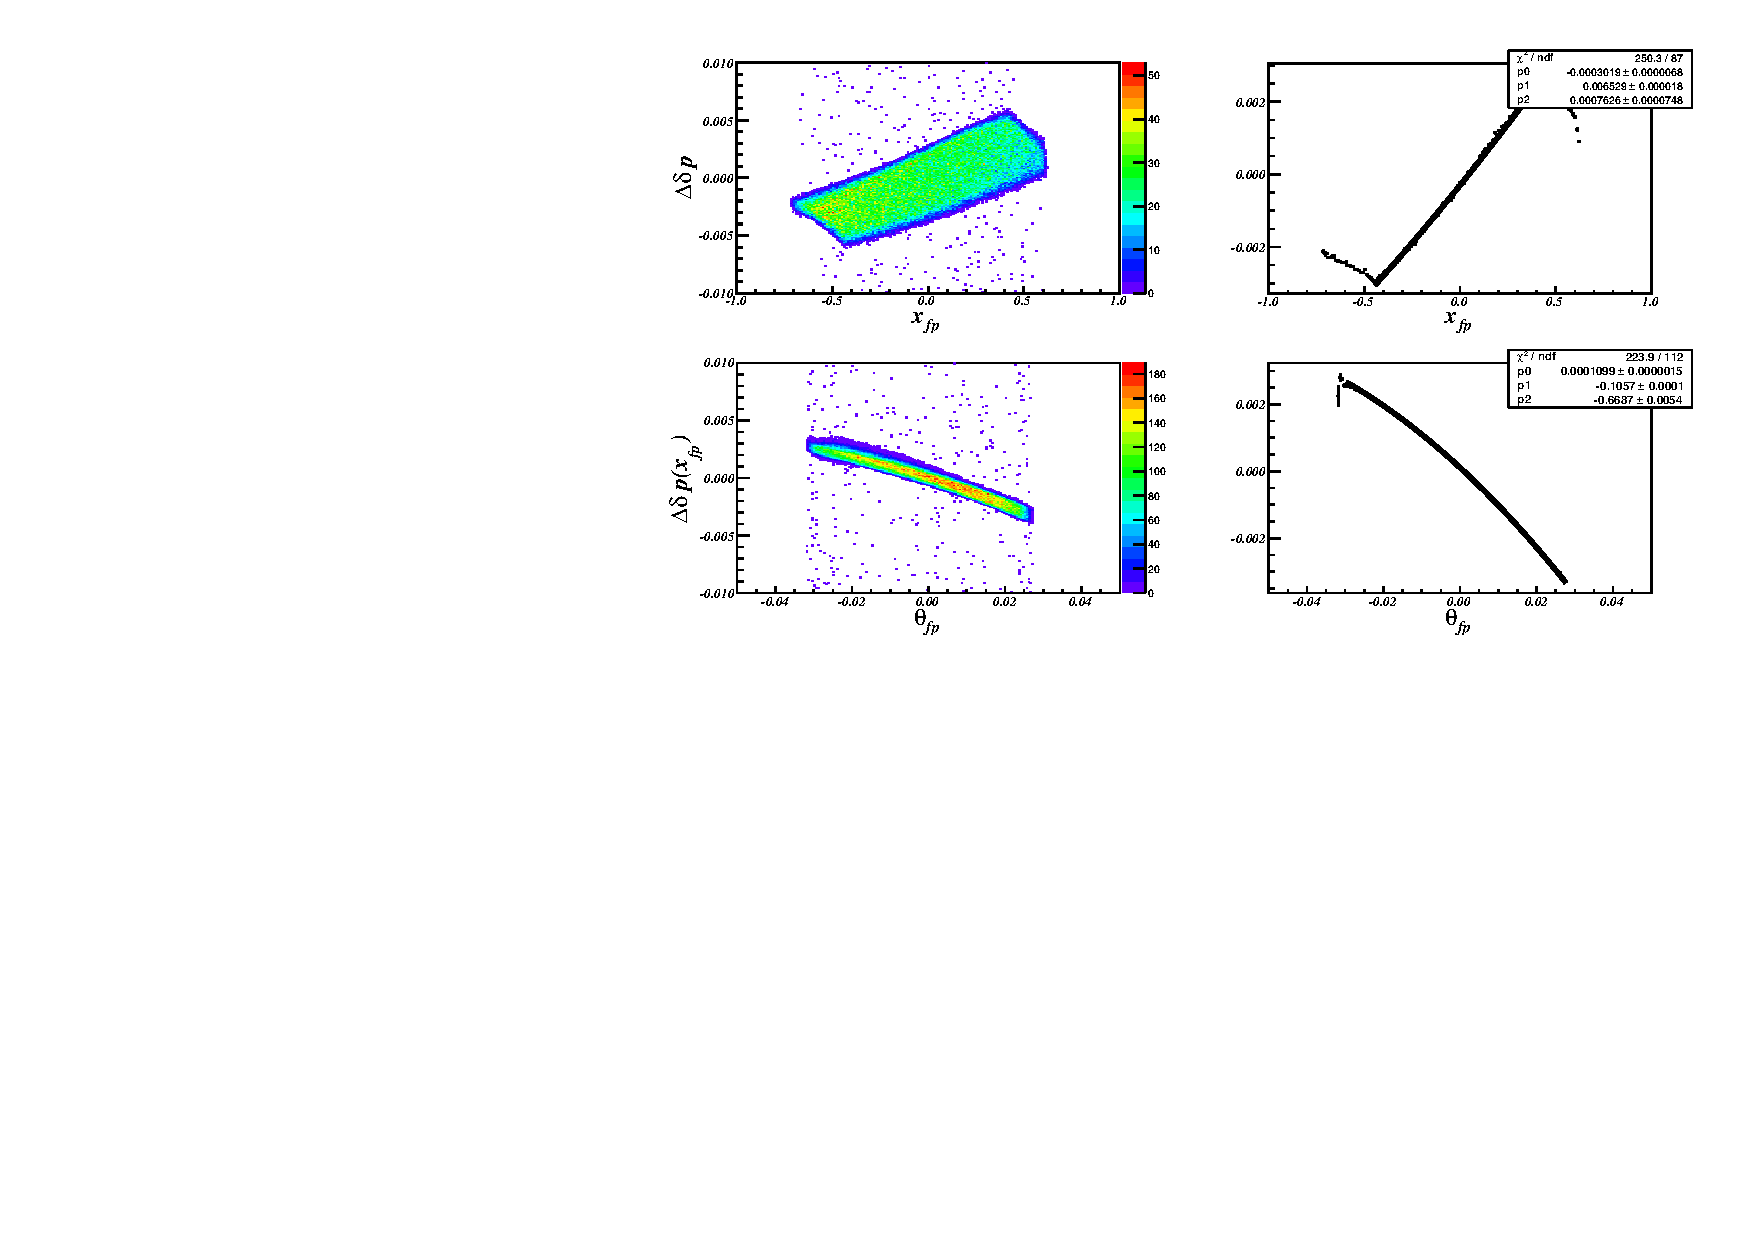
\includegraphics[type=pdf,ext=.pdf,read=.pdf,width=0.7\textwidth]{./figures/apend/DeltaCorr1_Kin31} 
    }
    \hfill
     \subfloat[$\Delta\delta p(y_{fp})$ .vs. $y_{fp}$ and $\phi_{fp}$]{
      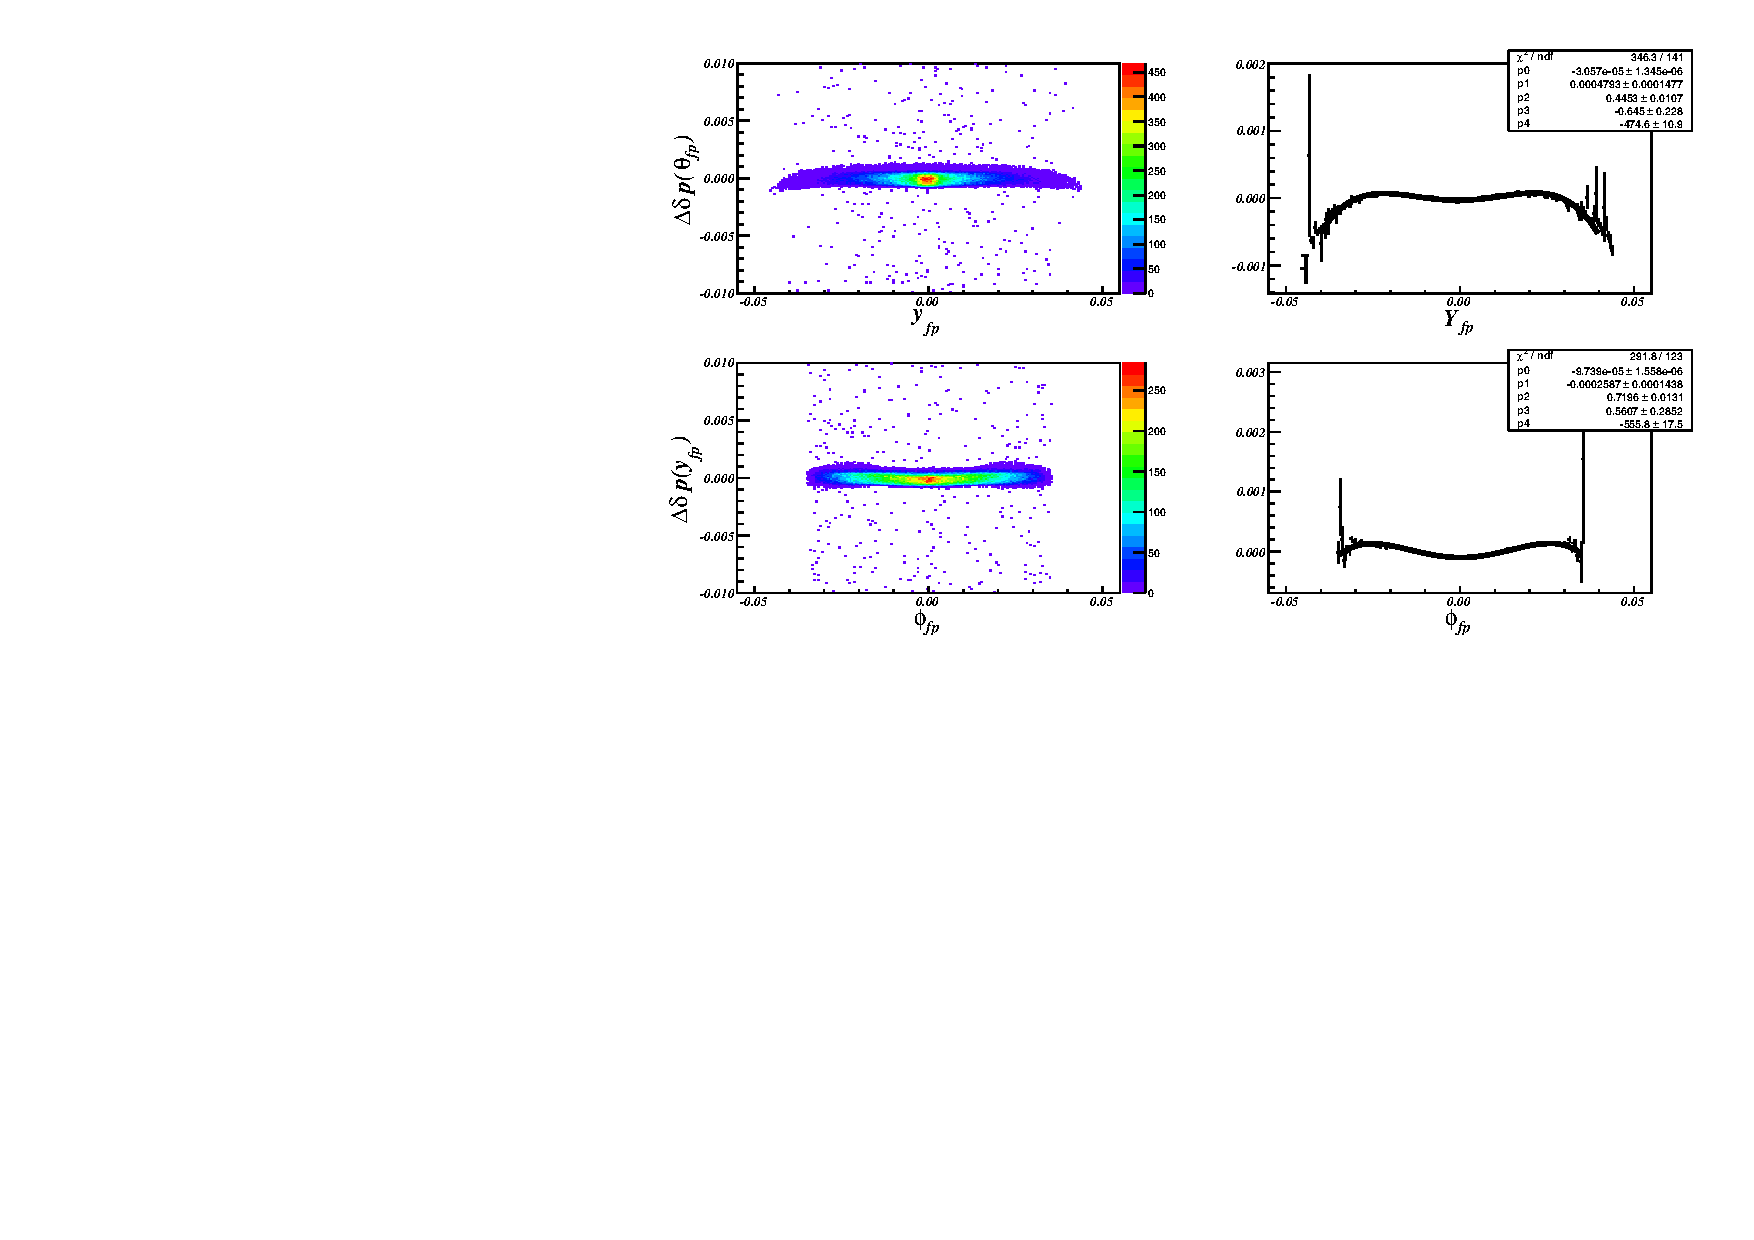
\includegraphics[type=pdf,ext=.pdf,read=.pdf,width=0.7\textwidth]{./figures/apend/DeltaCorr2_Kin31} 
    }
    \hfill
   \subfloat[$\Delta\delta p(\phi_{fp})$ .vs. $\delta p_{in}$]{
      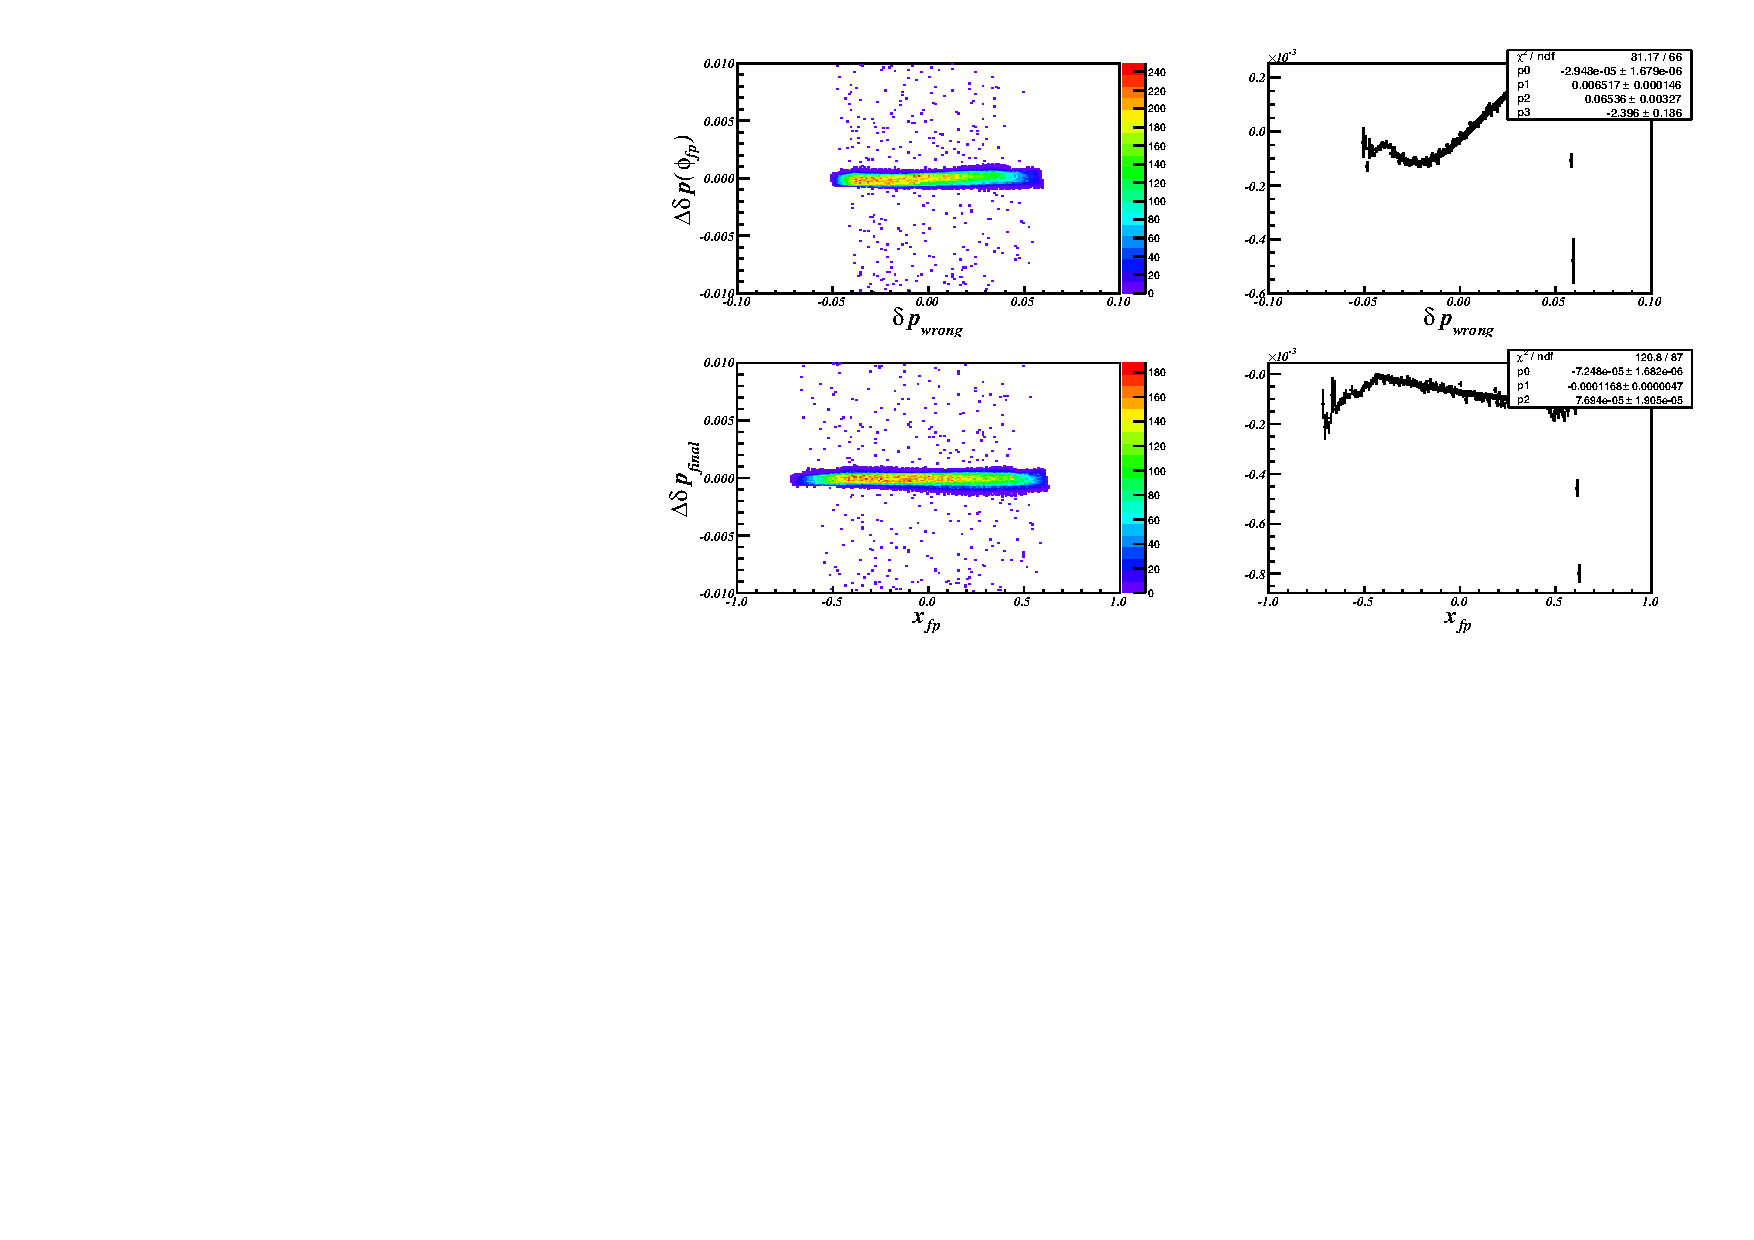
\includegraphics[type=pdf,ext=.pdf,read=.pdf,width=0.7\textwidth]{./figures/apend/DeltaCorr3_Kin31}
    }
    
    \caption[$\delta p$ correction function fitting]{\footnotesize{$\delta p$ correction function fitting with the focal plane variables. In each raw, the left is the 2-D histogram of $\Delta\delta p$ versus each fitting variable, while the right plot is the profile of the 2-D histogram, which is fitted with the polynomial function defined in Eq.~\eqref{deltap_corr_all}. The bottom two plots give the final result after applying all corrections.}}
    \label{deltap_fitting}
  \end{center}
\end{figure}

 Combining equations from Eq.~\eqref{deltap_corr_xfp} to Eq.~\eqref{deltap_corr_deltap}, Eq.~\eqref{dp_corr_func} leads to:
\begin{equation}
  \delta p_{cor}= \delta p_{in}+ f(x_{fp}, \theta_{fp}, y_{fp}, \phi_{fp}),
   \label{deltap_corr_all}
\end{equation}

 Fig.~\ref{deltap_fitting} shows the fitting result the distribution of $\Delta\delta p$ for each corrections. The final residual error, $\Delta\delta p(\delta p_{in})/\delta p_{cor}$, is close to $ 0.03\%$ (Fig.~\ref{deltap_final}) indicating that the mis-reconstructed momentum in the RQ3 has been corrected.
\begin{figure}[!ht]
 \begin{center}
  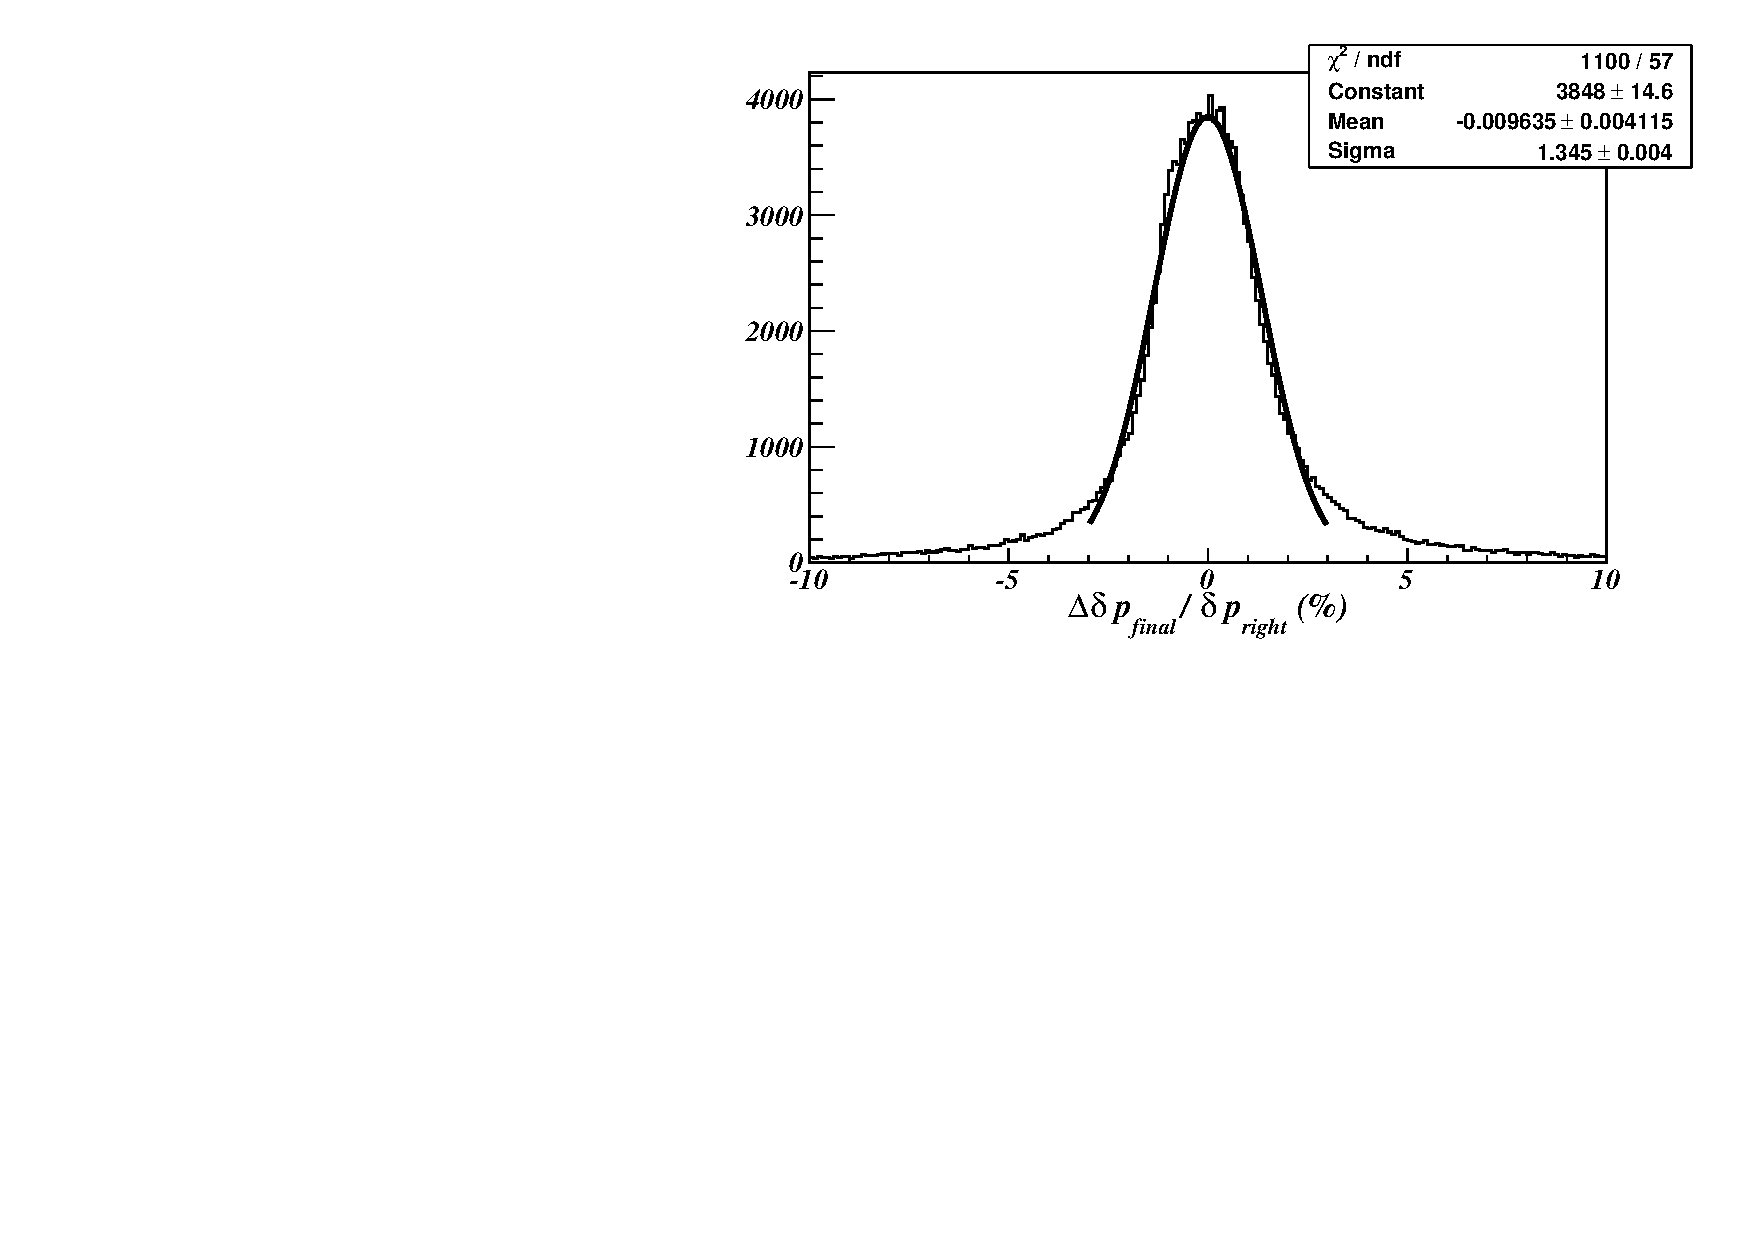
\includegraphics[type=pdf, ext=.pdf,read=.pdf,width=0.7\textwidth]{./figures/apend/DeltaCorr4_Kin31}
  \caption[The residual error of $\delta p$ correction function]{The residual error of $\delta p$ correction function. The momentum reconstruction value can be corrected with the error around $1.3\%$.}
  \label{deltap_final}
 \end{center}
\end{figure}
 \begin{figure}[!ht]
 \begin{center}
  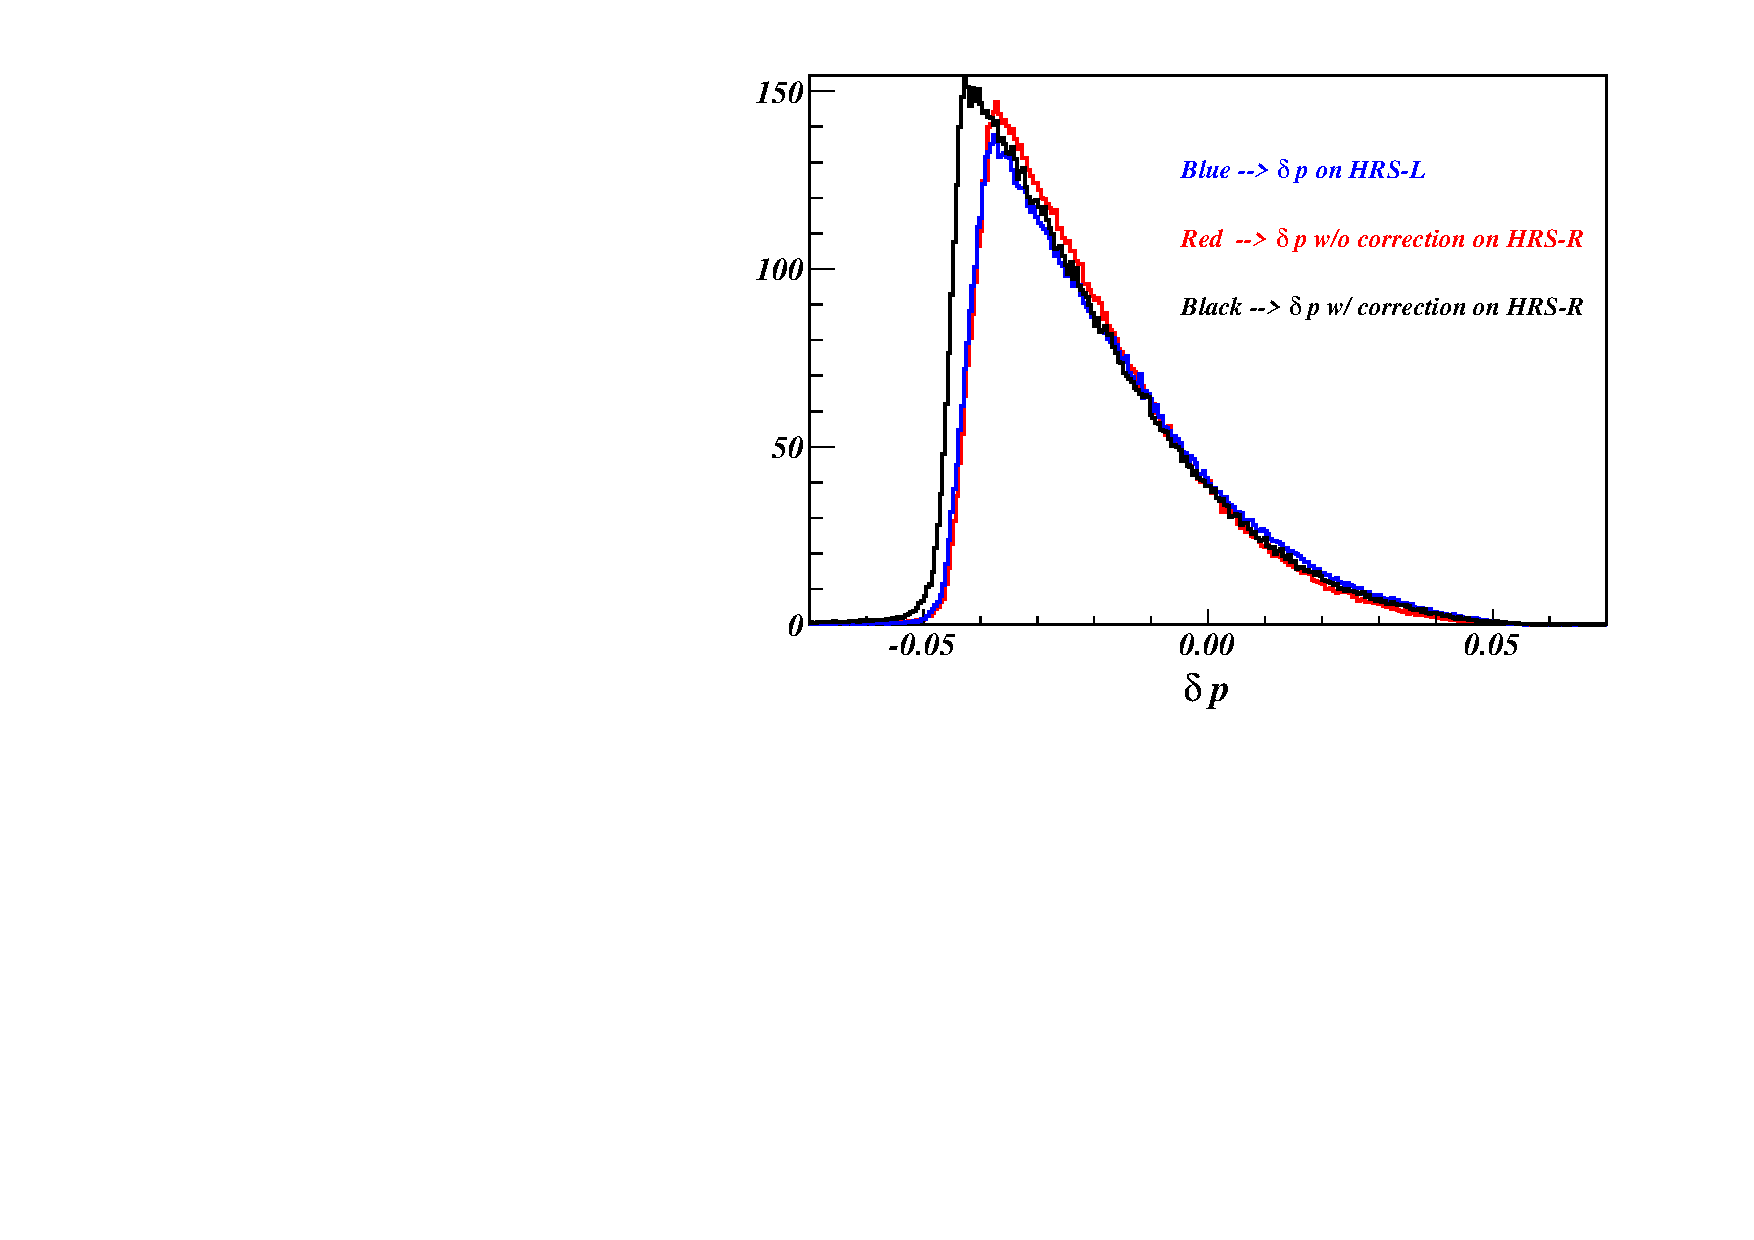
\includegraphics[type=pdf, ext=.pdf,read=.pdf,width=1.0\textwidth]{./figures/apend/DeltaP_Corr}
  \caption[$\delta p$ correction function applying on real data]{$\delta p$ correction function applying on real data. The data was taken on the carbon target with both HRSs at Kin5.0. The momentum distribution on HRS-R without the correction is different from the one on HRS-L (blue), which, however, agrees with the momentum distribution on HRS-R after the correction (black) at the central region. The $\delta p$ acceptance range on HRS-R is wider than the one on HRS-L, which can be explained by the defusing effect of the RQ3.}
  \label{deltap_corr_real}
 \end{center}
\end{figure}

 Eq.~\ref{deltap_corr_all} can be applied to the experimental data to correct the value of $\delta p$ for each event which is firstly reconstructed by the un-calibrated D-Terms in the HRS-R optics matrix. The performance of the correction can be examined by comparing the momentum distribution of the data taken in two HRSs with the same setting. Shown in Fig.~\ref{deltap_corr_real}, the momentum distribution on HRS-R should be identical to the one on HRS-L after applying the correction function, but its acceptance would be slightly wider than the one on HRS-L because of the defocussing effect of the RQ3.